\chapter{3D Dynamical Code}
\label{sc:dynamic}
\section{Discretisation of the dynamical equations}
\index{The hydrodynamic code}

% definitions pour les formules mathematiques
%\newcommand{\dep}[1]{\left( #1 \right) }
%\newcommand{\depb}[1]{\left[ #1 \right] }
%\newcommand{\depc}[1]{\left\{ #1 \right\} }
\newcommand{\deriv}[1]{\frac{\partial }{\partial #1} }
\def\abs#1{\left| #1 \right|}
\renewcommand{\-}[1]{$^{-#1}$}

% definitions pour la dynamique
\newcommand{\dt}[1]{\frac{\partial #1}{\partial t}}
\newcommand{\dsig}[1]{\deriv{\sigma} \dep{#1} }
\newcommand{\diverg}[1]{\vec{\nabla}.\dep{#1 \vec{V}} }
%\newcommand{\der}[2]{\frac{\partial #1 }{\partial #2} }
\def\ps{p_s}
\def\t{\theta}
\def\w{\dot{\sigma}}
\def\cp{C_p}
\def\rcp{\kappa}

%
%   ATTENTION  ne plait pas a latex2html (I don't know why)
%       de toutes facons inutile
%\def\p0{p_0}
%\def\s{ {\dep{\frac{p}{\p0}}}^{\rcp} }
%

\newcommand{\adv}[1]{\diverg{\ps #1} + \dsig{\ps #1 \dot{\sigma}} }

\def\sc#1{Section~\ref{sc:#1}}
\def\an#1{Annexe~\ref{an:#1}}
\def\ch#1{Chapitre~\ref{ch:#1}}
\def\fig#1{Fig.~\ref{fg:#1}}
\def\figs#1{Figs.~\ref{fg:#1}}
\def\eq#1{Eq.~\ref{eq:#1}}
\def\eqs#1{Eqs.~\ref{eq:#1}}
\def\tb#1{Table~\ref{tb:#1}}
%\newcommand{\av}[2]{{\overline{#1}}^{ #2 }}
%\newcommand{\avg}[1]{\left< #1 \right>}
\def\cd{C_D}
\def\dx{\delta_X}
\def\dy{\delta_Y}
\def\dz{\delta_Z}

\def\filtre{{\cal F}}
\def\uabs{\tilde{u}_{a}}
\def\err{\epsilon}
\def\dsig{\dz \sigma}
\def\psk{{\ps}^\kappa}
\def\ucov{\tilde{u}}
\def\vcov{\tilde{v}}
\def\ucont{\tilde{\ucov}}
\def\vcont{\tilde{\vcov}}
\def\cu{c_u}
\def\cv{c_v}
\def\h{\theta}
\def\pext{\tilde{p}_s}
\def\fext{f}
\def\K{\frac{1}{2}
\left( \av{\ucov \ucont}{X} + \av{\vcov \vcont}{Y} \right)}
\def\Z{\frac{\filtre\dep{\dx \vcov - \dy \ucov} + \fext}{\av{\pext}{X,Y}}}
\def\Zm{\frac{- \dy \ucov + \fext}{\av{\pext}{Y}}}

\newcommand{\glob}[1]{ \left< #1 \right> }

{\it Extrait de la note de Robert Sadourny, Phu Le Van et Fr\'ed\'eric
Hourdin, Laboratoire de M\protect\'et\protect{\'e}orologie Dynamique}.\\

[to be translated when I get the time...]

Le mod\`ele climatique du LMD est b\^ati, comme tous les
mod\`eles de circulation g\'en\'erale atmosph\'erique,
sur la r\'esolution num\'erique des {\'equations primitives
de la m\'et\'eorologie} d\'ecrites dans de nombreux
ouvrages~\cite{Holt:79}.
L'analyse pr\'esent\'ee ici a \'et\'e men\'ee sur la nouvelle
version de la dynamique du LMD \'ecrite par Phu Le Van~\cite{LeVa:89}
sur une formulation de Robert Sadourny.
Cette formulation diff\`ere de l'ancienne essentiellement
par deux points:
dans la nouvelle formulation, la r\'epartition des points en
longitude et en latitude peut \^etre chang\'ee arbitrairement.
L'autre modification porte sur la r\'epartition des points
aux p\^oles\footnote{Aux p\^oles sont calcul\'es:
le vent m\'eridien dans l'ancienne formulation et les variables
scalaires dans la nouvelle.}.

La coordonn\'ee  verticale du mod\`ele est la pression normalis\'ee
par sa valeur \`a la surface: $\sigma=p/\ps$.
On utilise en fait $\sigma$ aux niveaux inter-couches
et $s=\sigma^\kappa$ au milieu des couches.
On note $X$ et $Y$ les coordonn\'ees horizontales:

\begin{figure}
\begin{center}
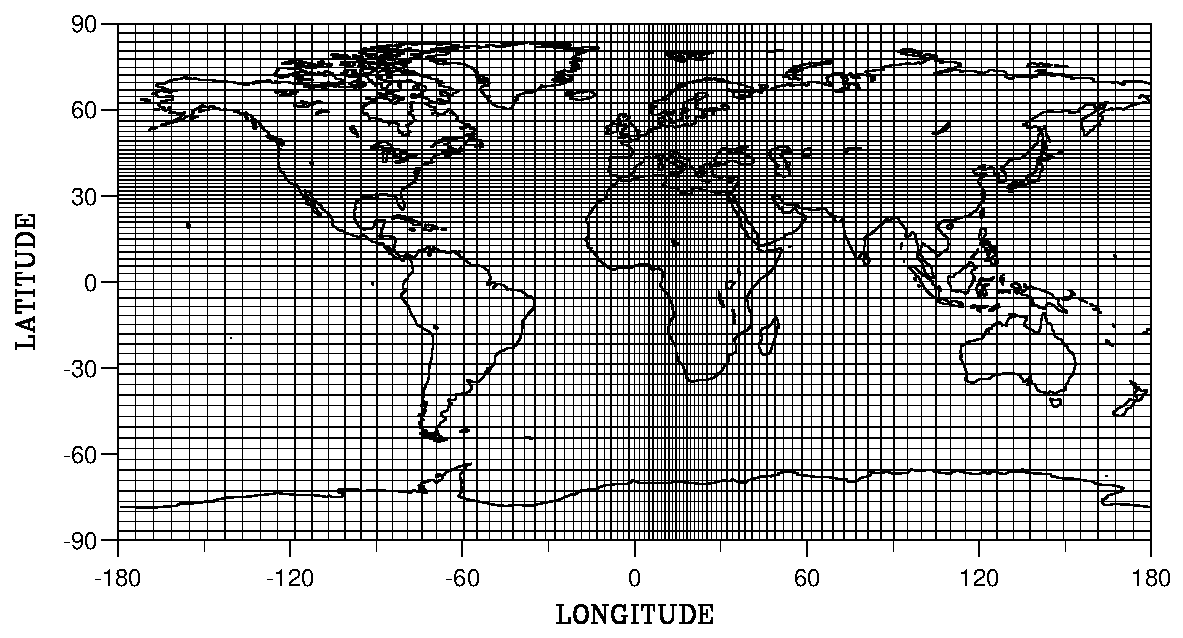
\includegraphics[width=13cm]{Fig/glob.eps}
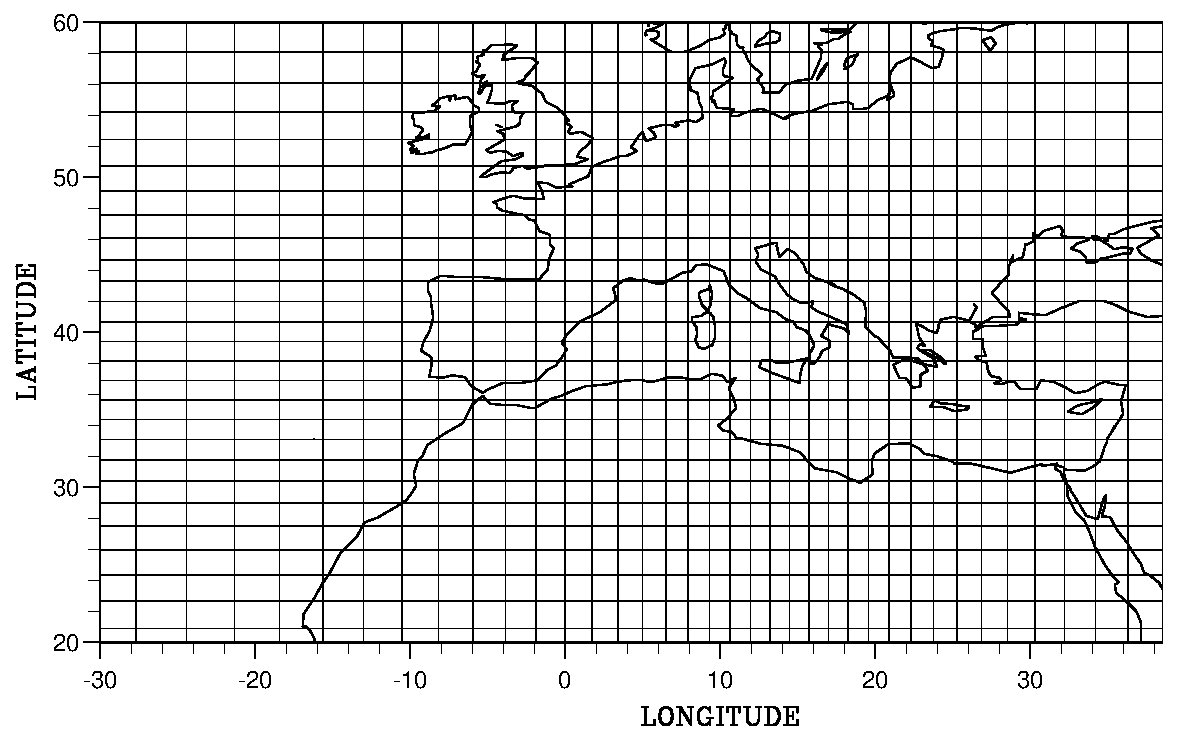
\includegraphics[width=10cm]{Fig/med.eps}
\caption{Grille obtenue avec 96 points en longitude et 73 en latitude et
un zoom d'un facteur 3 centr\'e sur la m\'edit\'erann\'ee (grille utilis\'ee au laboratoire par Ali Harzallah)\label{fg:zoom}}.
\end{center}
\end{figure}

$X$ (resp. $Y$) est une fonction biunivoque de la longitude $\lambda$
(resp. de la latitude $\phi$). Ces deux fonctions peuvent \^etre choisies
de fa\c{c}on arbitraire dans le mod\`ele LMDZ ce qui permet d'effectuer un
zoom sur une r\'egion du globe particuli\`ere. Une grille de ce type est montr\'ee
sur la Figure~\ref{fg:zoom}.
Les variables scalaires
(temp\'erature potentielle $\h = c_p T/\psk$, g\'eopotentiel $\Phi$
et pression de surface $\ps$) sont \'evalu\'ees aux points
correspondant \`a des couples de valeurs enti\`eres $(X,Y)=(i,j)$.
Les variables dynamiques sont d\'ecal\'ees par rapport aux variables
scalaires en utilisant une grille $C$ dans la d\'efinition de
Arakawa~\cite{Arak:77}: le vent zonal est calcul\'e
aux points $(X,Y)=(i+1/2,j)$ et  le vent
m\'eridien aux points $(X,Y)=(i,j+1/2)$.
La disposition des variables sur la grille est illustr\'ee sur la
Figure~\ref{fg:grille}.

\begin{figure}
\centerline{\framebox{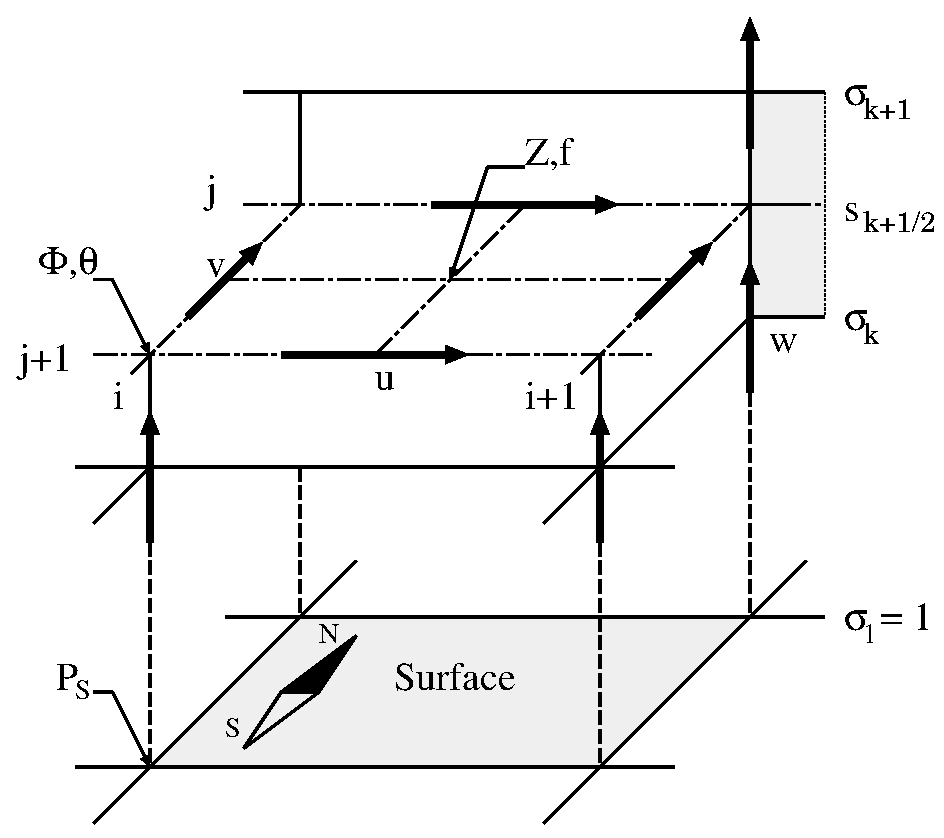
\includegraphics[width=0.6\textwidth]{Fig/grille.eps}}}
\caption{Disposition des variables dans la grille du LMD}
\label{fg:grille}
\end{figure}


On utilise en fait les composantes covariantes
($\ucov$ et $\vcov$) et contravariantes ($\ucont$ et $\vcont$)
du vent d\'efinies par
\begin{equation}
\begin{array}{llllllllll}
\ucov = \cu u & \mbox{et} & \ucont = u / \cu & \mbox{avec} &
\cu = a \cos{\phi} \left( d\lambda/dX \right)  \\
\vcov = \cv v & \mbox{et} & \vcont = v / \cv & \mbox{avec} &
\cv = a \left( d\phi / dY \right)
\end{array}
\end{equation}
%
o\`u $u$ et $v$ sont les composantes physiques du vecteur vent
horizontal.
On introduit \'egalement:
%
\paragraph{la pression extensive:}
$\pext$ (pression au sol multipli\'ee
par l'aire de la maille).
%
\paragraph{les trois composantes du flux de masse:}
\begin{equation}
U=\av{\pext}{X} \ucont ,\  V= \av{\pext}{Y} \vcont \  \mbox{et} \
W= \pext \dot{\sigma}
\ \mbox{avec}\ \dot{\sigma}=\frac{d\sigma}{dt}
\end{equation}
%
\paragraph{le facteur de Coriolis multipli\'e par l'aire de la maille:}
$\fext=2\Omega \sin{\phi} \cu \cv$\\
o\`u $\Omega$ est la vitesse de rotation de la plan\`ete.
%
\paragraph{la vorticit\'e potentielle absolue:}
\begin{equation}
Z=\Z
\end{equation}
%
\paragraph{l'\'energie cin\'etique}
\begin{equation}
K=\K
\end{equation}\\
%
La notation $\delta X$ signifie simplement qu'on
effectue la diff\'erence entre deux points cons\'ecutifs
suivant la direction $X$.
La notation $\av{a}{X}$ signifie qu'on prend la moyenne arithm\'etique
de la quantit\'e $a$ suivant la direction $X$. $\filtre$ est un filtre longitudinale appliqu\'e dans les r\'egions polaires.
Les \'equations discr\'etis\'ees sont \'ecrites sous la forme
suivante:
\paragraph{\'equations du mouvement:}
\begin{equation} \label{eq:u1}
\dt{\ucov} -
\av{Z}{Y} \av{V}{X,Y}
+ \dx \filtre\dep{\Phi + K}
+s \av{\h}{X} \dx \filtre\dep{\psk}
- \frac{\av{\uabs}{Y,Y} \dz \av{W}{X} }
{\av{\pext}{X} \dsig }
+ \frac{\dz \left( \av{W}{X} \av{\uabs}{Z} \right) }
{\av{\pext}{X} \dsig}
=S_{\ucov}
\end{equation}
o\'u $\uabs$ est la composante zonale covariante
du vecteur vent absolu:
$\uabs=\ucov+\cu a \Omega \cos{\phi}$ et
\begin{equation} \label{eq:v1}
\dt{\vcov} + \av{Z}{X} \av{U}{X,Y} + \dy \filtre\dep{\Phi + K}
+s \av{\h}{Y} \dy \filtre\dep{\psk}
- \frac{\av{\vcov}{X,X} \dz \av{W}{Y} }
{\av{\pext}{Y} \dsig}
+ \frac{\dz \left( \av{W}{Y} \av{\vcov}{Z} \right) }
{\av{\pext}{X} \dsig}
=S_{\vcov}
\end{equation}
%
\paragraph{\'equation thermodynamique:}
%
\begin{equation}
\label{eq:thermo}
\dt{\dep{\pext \h}}
+\filtre\depb{\dx \dep{\av{\h}{X}U} +\dy \dep{\av{\h}{Y}V} }
+\frac{\dz \dep{\av{\h}{Z} W}}{\dz \sigma}=S_\h
\end{equation}
%
\paragraph{\'equation hydrostatique:}
\begin{equation}
\dz \Phi=-\ps^\rcp  \av{\h}{z} \dz s
\end{equation}
%
\paragraph{\'equations de continuit\'e:}
%
\begin{equation}
\label{eq:cont1}
\dt{\ps}  = \filtre\depb{\sum_z{\dz \sigma \dep{\dx U+ \dy V}}}
\end{equation}
\begin{equation}
\label{eq:cont2}
\dz W   = -\dz \sigma \depb{\filtre\dep{\dx U+ \dy V} + \dt{\ps}}
\end{equation}
%
On a not\'e $S$ les termes sources dans les diff\'erentes \'equations.
Dans ces termes sources, on distingue 1) d'une part les param\'etrisations physiques mentionn\'ees plus haut et qui font intervenir pour une maille donn\'ee du mod\`ele, tous les points situ\'es sur une m\^eme verticale mais ceux-l\`a seulement; 2) les op\'erateurs de dissipation horizontale, cens\'es rendre compte des \'echanges entre \'echelles explicitement repr\'esent\'ees dans le mod\`ele et \'echelles sous-mailles. Ces op\'erateurs ont la structure de Laplaciens agissant sur des plans horizontaux c'est \`a dire qu'il font intervenir un voisin de chaque c\^ot\'e dans les deux directions horizontales. Cet op\'erateur est g\'en\'eralement it\'er\'e pour le rendre plus s\'electif en \'echelle (plus on it\`ere un laplacien et plus son effet sur les petites \'echelles devient important relativement).

\section{High latitude filters}

{\it Extract adapted from Forget et al. [1999]}\\

At high latitude a filter is applied near
the singularity in the grid at the pole
in order to satisfy the Courant-Friedrichs-Lewy numerical
stability criterion without going to an excessively
small timestep. In the original version of the dynamical code
a classical Fourier filter was used,  but
we found that because the Martian polar
atmosphere appears to be much more dynamically unstable than the Earth's
polar atmosphere, a more efficient formulation (based on the
grouping of adjacent gridpoints together)  was necessary
to avoid numerical instability. \\

{\it In practice the following technique is used in the subroutine called {\em groupeun.F} :
\begin{itemize}
\item The points are grouped in packets of $2^{\mbox{ngroup}}$
      at the poles(e.g. {\bf ngroup}=3 $\rightarrow$ packets of 8),
 then $2^{\mbox{ngroup-1}}$,
      $2^{\mbox{ngroup-2}}$, etc. in the lower latitudes moving away from the pole

   \item The higher {\bf ngroup} is, the more efficient the smoothing is, and the more stable the model.

\item   BUT, {\bf iim} must be divisible by $2^{\mbox{ngroup}}$ !!!


\end{itemize}

}


\section{Dissipation}

{\it Extract adapted from Forget et al. [1999]}\\

In the LMD grid point model,
nonlinear interactions between explicitly resolved scales
and subgrid-scale processes are
parameterized by applying a scale-selective horizontal
dissipation operator
based on an $n$ time iterated Laplacian $\Delta^{n}$.
For the grid point model, for instance, this can be written
${\partial q}/{\partial t} = ([-1]^{n}/ {\tau_{\mbox{\scriptsize
diss}}})
(\delta x)^{2n} \Delta^{n} q$
where $\delta x$ is the smallest horizontal distance represented in the
model and $\tau_{\mbox{\scriptsize diss}}$ is the dissipation timescale
for a st
ructure of scale
$\delta x$.
These operators are necessary to ensure the grid point model
numerical stability.
In practice, the operator is
separately applied to (1)~potential temperature, (2)~the divergence of
the flow,
and (3)~its vorticity.
We respectively use  $n=2$, $n=1$, and $n=2$ in the grid point model.\\

{\it Note: In practice,
values of $n$ and $\tau_{\mbox{\scriptsize diss}}$
are adjustable and prescribed at the beginning of each run, in run definition file ``run.def'' (cf.~\ref{vb:run.def}) }

\section{Sponge layer}

{\it Extract adapted from Forget et al. [1999]}\\

In the upper levels a sponge layer is also used in both models
in an attempt to reduce
spurious reflections of vertically propagating waves from the model top.
Unlike the traditional Rayleigh friction formulation,
this operates as a linear drag
 solely on the eddy components of the vorticity and divergence
fields and is not scale-selective.  The timescales on which it operates
are
typically half a day, 1 day,  and 2 days
 at the three uppermost levels, respectively. \\

{\it Note: the sponge layer ``timescale'' values and their extensions in altitude
are adjustable and prescribed at the beginning of each run, in run definition file ``run.def'' (cf.~\ref{vb:run.def}) }







